\chapter{Quality Control with Six Sigma and R Analytics}

Good data is the key to making smart decisions in climate and agriculture. If the data has mistakes, missing values, or doesn't match real-world conditions, it can lead to wrong predictions and poor planning. Quality Control (QC) helps catch and fix these problems so that the data can be trusted and used confidently.

In this chapter, we introduce a simple and structured way to check and improve data quality using the Six Sigma method. We also show how these techniques can be applied using the R programming language.

\section{What is Data Quality?}

Data quality refers to how accurately and reliably a dataset reflects the real world. High-quality data is complete, correct, consistent, and up to date. It forms the foundation for meaningful analysis, sound decisions, and effective planning.

When data is accurate and trustworthy, it can lead to better outcomes whether it's in business, research, public policy, or everyday problem-solving. But when data is missing, incorrect, or inconsistent, it can lead to misunderstandings, poor decisions, and costly mistakes.

For example, in climate data, this means temperature or rainfall measurements should be accurate and recorded properly over time. High-quality data helps in making better decisions like predicting weather patterns or managing resources effectively. Poor-quality data, such as missing values or incorrect measurements, can lead to wrong conclusions and costly mistakes.

\section{What is Quality Control (QC)?}

Quality Control is the process of checking and correcting data to ensure it is reliable and useful for analysis.

QC involves steps like:
\begin{itemize}
  \item Detecting missing, extreme, or unusual values
  \item Measuring how much data varies from what is expected
  \item Fixing problems by correcting errors or filling gaps
  \item Setting up ongoing monitoring to catch future issues
\end{itemize}

Taking our climate dataset as a reference, here are some practical examples:

\begin{itemize}
  \item Sometimes, a temperature sensor may report impossible values—such as 50°C during winter or -100°C—which clearly indicate errors needing correction.
  \item Missing data can occur when a rainfall gauge fails to record measurements for several days. This gap must be addressed to avoid biased rainfall averages.
  \item Occasionally, sudden spikes or drops in data—for example, a sudden 10°C jump in temperature from one day to the next—may not align with realistic weather patterns and should be flagged for review.
\end{itemize}

QC processes identify these issues, then either correct them (by imputing missing values or adjusting errors) or exclude problematic data to ensure the dataset reflects reality as closely as possible.

\section{Why Is This Important?}

Without QC, poor-quality data can lead to incorrect or misleading conclusions. For example:

\begin{itemize}
  \item Overestimated temperatures may falsely indicate warming trends, affecting climate change studies.
  \item Missing or incorrect rainfall data can lead to wrong predictions about droughts or floods, impacting disaster preparedness.
  \item Inaccurate data can cause flawed agricultural advice, such as mistimed planting or irrigation schedules, resulting in crop loss.
\end{itemize}

By applying QC, we improve data accuracy and build trust in analysis outcomes, enabling better decisions based on solid evidence.

\section{What is Six Sigma?}

Six Sigma is a structured, statistics-driven approach designed to improve quality and reduce errors in processes. Originally created for manufacturing to minimize defects, Six Sigma has since been adopted widely in data analytics, healthcare, finance, and many other fields.

The core idea is to identify problems clearly, measure performance accurately, analyze causes, implement improvements, and then maintain the gains—ensuring high-quality outputs every time.

Six Sigma follows five key phases, known as DMAIC:

\begin{table}[h!]
\centering
\begin{tabular}{|l|p{5cm}|p{4cm}|p{4cm}|}
\hline
\textbf{Phase} & \textbf{Core Question} & \textbf{Example (Climate Data)} & \textbf{Key Methods Used} \\
\hline
Define & What problem are we trying to solve? & “Some rainfall data seem inconsistent.” & SIPOC diagram, Project Charter, Voice of Customer (VOC) \\
\hline
Measure & How is the data performing now? & Summarize and check for missing or outlier values. & Descriptive statistics, Control charts, Missing value analysis \\
Analyze & Why are these problems happening? & Identify faulty sensors or data entry errors. & Root Cause Analysis, Pareto Chart, Correlation Analysis, Fishbone Diagram \\
\hline
Improve & How can we fix the issues? & Replace missing values or correct wrong entries. & Hypothesis Testing, Data Imputation, Regression, Design of Experiments (DoE) \\
\hline
Control & How do we keep the data clean moving forward? & Set up monitoring charts or alerts for new issues. & Statistical Process Control (SPC), Control Charts, Dashboards, Check Sheets \\
\hline
\end{tabular}
\caption{Six Sigma DMAIC Phases Applied to Climate Data}
\end{table}

Below, we explore each phase in detail, along with practical implementation using R programming in the context of climate data.

\subsection*{1. Define – Understand the Problem}

\textbf{Purpose:} This phase focuses on clearly identifying the problem and defining the objectives of the improvement effort. It ensures clarity of purpose and aligns stakeholders on what success looks like.

\textbf{Activities May Include:}
\begin{itemize}
  \item Identifying the problem or variation in data
  \item Defining goals and scope
  \item Creating a project charter
\end{itemize}

\textbf{Example (Climate Context):} 

We suspect that daily temperature data collected from 1980 to 2020 may contain sudden shifts or unstable patterns that could mislead seasonal predictions.

\subsection*{2. Measure}

\textbf{Purpose:} The goal of the measure phase is to collect relevant data and understand the current performance or quality of the process. This involves evaluating the data’s completeness, variability, and reliability.

\textbf{Key Techniques:}
\begin{itemize}
  \item Summary statistics (mean, median, standard deviation)
  \item Outlier detection
  \item Control charts to assess process stability
\end{itemize}

\textbf{R Implementation:} We use a Control Chart to track whether the daily average temperature stayed within control limits (normal variation range).

\begin{verbatim}
# Calculate mean and standard deviation
mean_temp <- mean(df_climate$Temp_2m, na.rm = TRUE)
sd_temp <- sd(df_climate$Temp_2m, na.rm = TRUE)

# Create the control chart
ggplot(df_climate, aes(x = Date, y = Temp_2m)) +
  geom_line(color = "steelblue") +
  geom_hline(yintercept = mean_temp, color = "green", 
  linetype = "dashed", size = 1, alpha = 0.8) +
  geom_hline(yintercept = mean_temp + 3 * sd_temp, color = "red", 
  linetype = "dashed", size = 1, alpha = 0.8) +
  geom_hline(yintercept = mean_temp - 3 * sd_temp, color = "red", 
  linetype = "dashed", size = 1, alpha = 0.8) +
  scale_x_date(date_breaks = "1 year", date_labels = "%Y") +
  labs(title = "Control Chart for Temperature at 2m Height (1980-2020)",
       x = "Year",
       y = "Temperature (°C)") +
  theme_minimal() +
  theme(axis.text.x = element_text(angle = 45, hjust = 1))
\end{verbatim}

% Figure here-----------------------------
\begin{figure}[h]
\centering
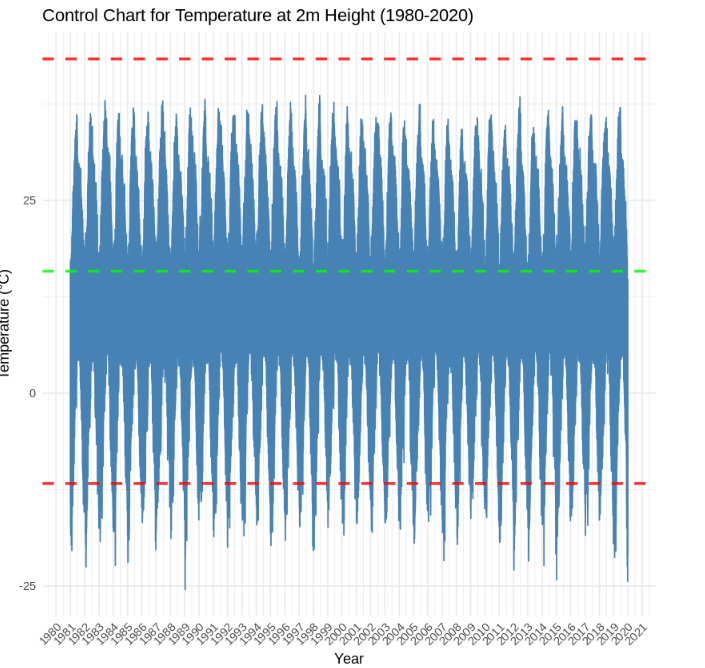
\includegraphics[width=0.5\textwidth]{figures/control_chart.png}
\caption{Control Chart for Temperature at 2m Height (1980-2020)}
\end{figure}

\textbf{Interpretation:} The plot shows the temperature over time with control limits (mean ± 3 standard deviations). Points outside the red dashed lines indicate abnormal data points potentially caused by sensor faults or extreme weather.

\subsection*{3. Analyze}

\textbf{Purpose:} This phase aims to determine the root causes of the problems detected in the measurement phase. It involves deeper data analysis to uncover patterns or sources of variation.

\textbf{Key Techniques:}
\begin{itemize}
  \item Hypothesis testing
  \item Variance analysis by group
  \item Correlation or trend analysis
\end{itemize}

\textbf{R Implementation:} To determine whether there is a statistically significant difference in temperature between seasons by using hypothesis testing (T-test):\\

\textbf{Hypothesis Testing}
\begin{itemize}
  \item Null Hypothesis (H0): No significant difference in mean temperature between summer and winter.
  \item Alternative Hypothesis (H1): Significant difference in mean temperature between summer and winter.
\end{itemize}

\begin{verbatim}
summer <- df_climate[df_climate$Season == "Summer", "Temp_2m"]
winter <- df_climate[df_climate$Season == "Winter", "Temp_2m"]

t_test <- t.test(summer, winter)
print(t_test)
\end{verbatim}

% figure here--------------------------
\begin{figure}[h]
\centering
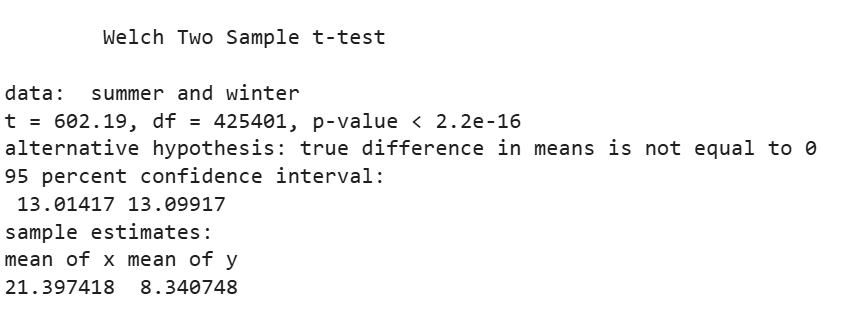
\includegraphics[width=0.7\textwidth]{figures/welch.png}
\caption{Welch Two Sample t-test}
\end{figure}
\textbf{Interpretation:}

\begin{itemize}
    \item The \emph{p}-value is extremely small ($< 2.2 \times 10^{-16}$), which is far below the standard threshold of $0.05$.
    
    \item This result allows you to confidently reject the null hypothesis.
    
    \item The mean temperature difference between summer and winter is approximately $13^\circ$C, with summer being significantly warmer.
\end{itemize}

\textbf{Detecting Anomalies (Outliers):}

We check for daily temperature spikes.

\begin{verbatim}
outliers <- df_climate %>%
  filter(Temp_2m > mean_temp + 3*sd_temp | Temp_2m < mean_temp - 3*sd_temp)

# Print the number of outlier rows
cat("Number of outliers:", nrow(outliers), "\n")
\end{verbatim}

\textbf{Expected output:} Number of outliers: 4973

\subsection*{4. Improve}

\textbf{Purpose:} This phase focuses on developing and implementing solutions that directly address the root causes identified in the analysis. The goal is to improve data quality, reduce variation, or make the process work more smoothly and efficiently.

\textbf{Key Techniques:}
\begin{itemize}
  \item Data cleaning and imputation
  \item Smoothing techniques
  \item Process optimization
\end{itemize}

\textbf{R Implementation:} A rolling average can be used to smooth temperature data and detect long-term trends.

\begin{verbatim}
library(zoo)
# Compute 30-day rolling average

df_climate$Temp_Smooth <- rollmean(
  df_climate$Temp_2m, 
  k = 30, 
  fill = NA
  )

# Plot only the smoothed temperature line
plot(df_climate$Date,df_climate$Temp_Smooth,
     type = 'l',
     col = 'blue', 
     lwd = 2,
     xlab = "Date", 
     ylab = "Smoothed Temperature (°C)",
     main = "30-Day Rolling Average of Temperature"
) 
\end{verbatim}
\clearpage
% figure here--------------------------
\begin{figure}[h]
\centering
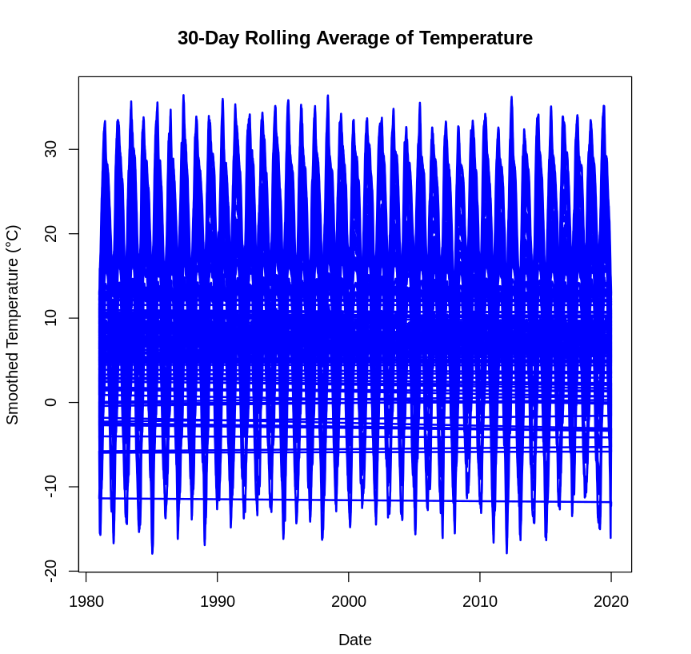
\includegraphics[width=0.4\textwidth]{figures/rolling_avg.png}
\caption{30-Day Rolling Average of Temperature}
\end{figure}

\textbf{Interpretation:} This plot reduces short-term fluctuations (noise), making it easier to observe underlying seasonal patterns or gradual climatic shifts.

\subsection*{5. Control}

\textbf{Purpose:} After improvements have been implemented, the control phase ensures that these gains are sustained over time. Monitoring mechanisms are set up to detect any new issues or deviations.

\textbf{Key Techniques:}
\begin{itemize}
  \item Continuous control charts
  \item Threshold alerts
  \item Rolling performance metrics
\end{itemize}

\textbf{R Implementation:} We now maintain the improvements by regularly checking:\\

\textbf{a. KPI: Extreme Heat Days}
\begin{verbatim}
extreme_days <- df_climate %>% filter(Temp_2m > 35)
extreme_percent <- (nrow(extreme_days) / nrow(df_climate)) * 100
cat(sprintf("Extreme Heat Days: %.2f%%\n", extreme_percent))

Expected output: Extreme Heat Days: 0.13%
\end{verbatim}

\textbf{b. Monthly Monitoring Chart}

\begin{verbatim}
df_climate$Month <- format(df_climate$Date, "%Y-%m")

monthly_avg <- df_climate %>%
  group_by(Month) %>%
  summarise(Monthly_Temp = mean(Temp_2m, na.rm = TRUE))

ggplot(monthly_avg, aes(x = as.Date(paste0(Month, "-01")), y = Monthly_Temp)) +
  geom_line(color = "darkgreen") +
  labs(title = "Monthly Average Temperature Monitoring",
       x = "Month", y = "Temp (°C)") +
  scale_x_date(date_breaks = "1 year", date_labels = "%Y") +
  theme(axis.text.x = element_text(angle = 45, hjust = 1))
\end{verbatim}

% figure here--------------------------
\begin{figure}[h]
\centering
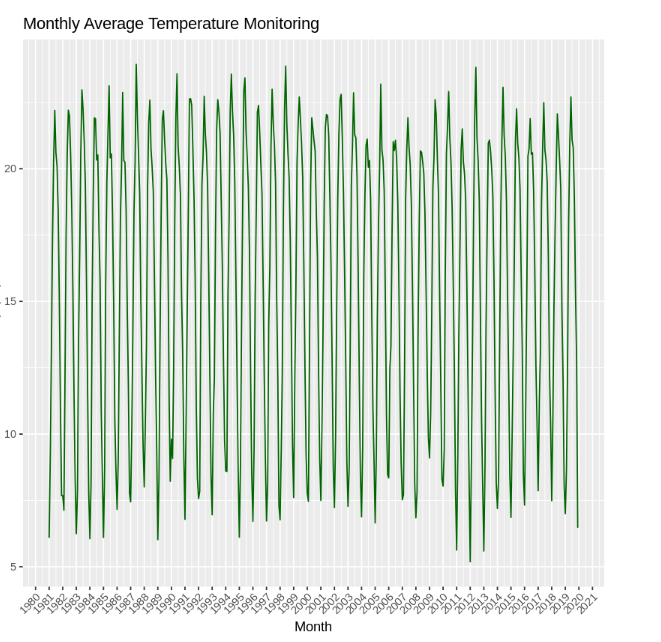
\includegraphics[width=0.5\textwidth]{figures/monitoring_chart.png}
\caption{Monthly Average Temperature Monitoring}
\end{figure}

\textbf{Interpretation:} This time series plot helps monitor temperature trends over months, allowing early detection of unusual patterns or shifts.

\section{Why Use Six Sigma in Data Analytics?}

Applying Six Sigma offers several benefits:

\begin{itemize}
  \item Catch data errors early: Fix problems before they affect results.
  \item Improve model accuracy: Better data means more reliable forecasts and analyses.
  \item Ensure consistency: Use the same quality standards across different data sources.
  \item Build trust: Transparent, documented methods increase confidence in data-driven decisions.
\end{itemize}

\section*{Let’s Think!}

Think about a dataset you’ve worked with. Can you identify any data quality problems that might benefit from the DMAIC approach? Here are some prompts to reflect on:

\begin{itemize}
  \item Have you ever found missing or suspicious values in your data? What did you do?
  \item How do you check whether your data matches what you expect?
  \item What methods have you used to fix or handle errors or gaps?
  \item Do you have any ways to monitor data quality regularly?
\end{itemize}
